\section{Writing your first piece of \LaTeX}

The first step is to create a new \LaTeX\ project. You can do this on your own computer by creating a new .tex file; alternatively, you can \href{https://www.overleaf.com/learn/how-to/Creating_a_document_in_Overleaf}{start a new project in Overleaf}.

Let’s start with the simplest working example, which can be opened directly in Overleaf:

\begin{tcolorbox}
\begin{verbatim}
    \documentclass{article}
    \begin{document}
    First document. This is a simple example, with no 
    extra parameters or packages included.
    \end{document}
\end{verbatim}
\end{tcolorbox}

This example produces the following output:

\begin{mdframed}
\-\hspace{20pt}First document. This is a simple example, with no 
extra parameters or packages included.
\end{mdframed}

You can see that \LaTeX\ has automatically indented the first line of the paragraph, taking care of that formatting for you. Let’s have a closer look at what each part of our code does.

The first line of code, \verb|\documentclass{article}|, declares the document type known as its class, which controls the overall appearance of the document. Different types of documents require different classes; i.e., a CV/resume will require a different class than a scientific paper which might use the standard LATEX article class. Other types of documents you may be working on may require different classes such as book or report. To get some idea of the many \LaTeX\ class types available, \href{https://www.ctan.org/topic/class}{visit the relevant page on CTAN (Comprehensive TeX Archive Network)}.

Having set the document class, our content, known as the body of the document, is written between the \verb|\begin{document}| and \verb|\end{document}| tags. After opening the example above, you can make changes to the text and, when finished, view the resulting typeset PDF by \emph{recompiling the document}. To do this in Overleaf, simply hit \textbf{Recompile}, as demonstrated in \href{https://videos.ctfassets.net/nrgyaltdicpt/6yo2PA5aMV3OEZl5NtZKWu/54395f569b830b8183b5e0058d5bc0cc/LL30recompile.mp4}{this brief video clip}.

Any Overleaf project can be configured to recompile automatically each time it is edited: click the small arrow next to the \textbf{Recompile} button and set \textbf{Auto Compile} to \textbf{On}, as shown in the following screengrab:

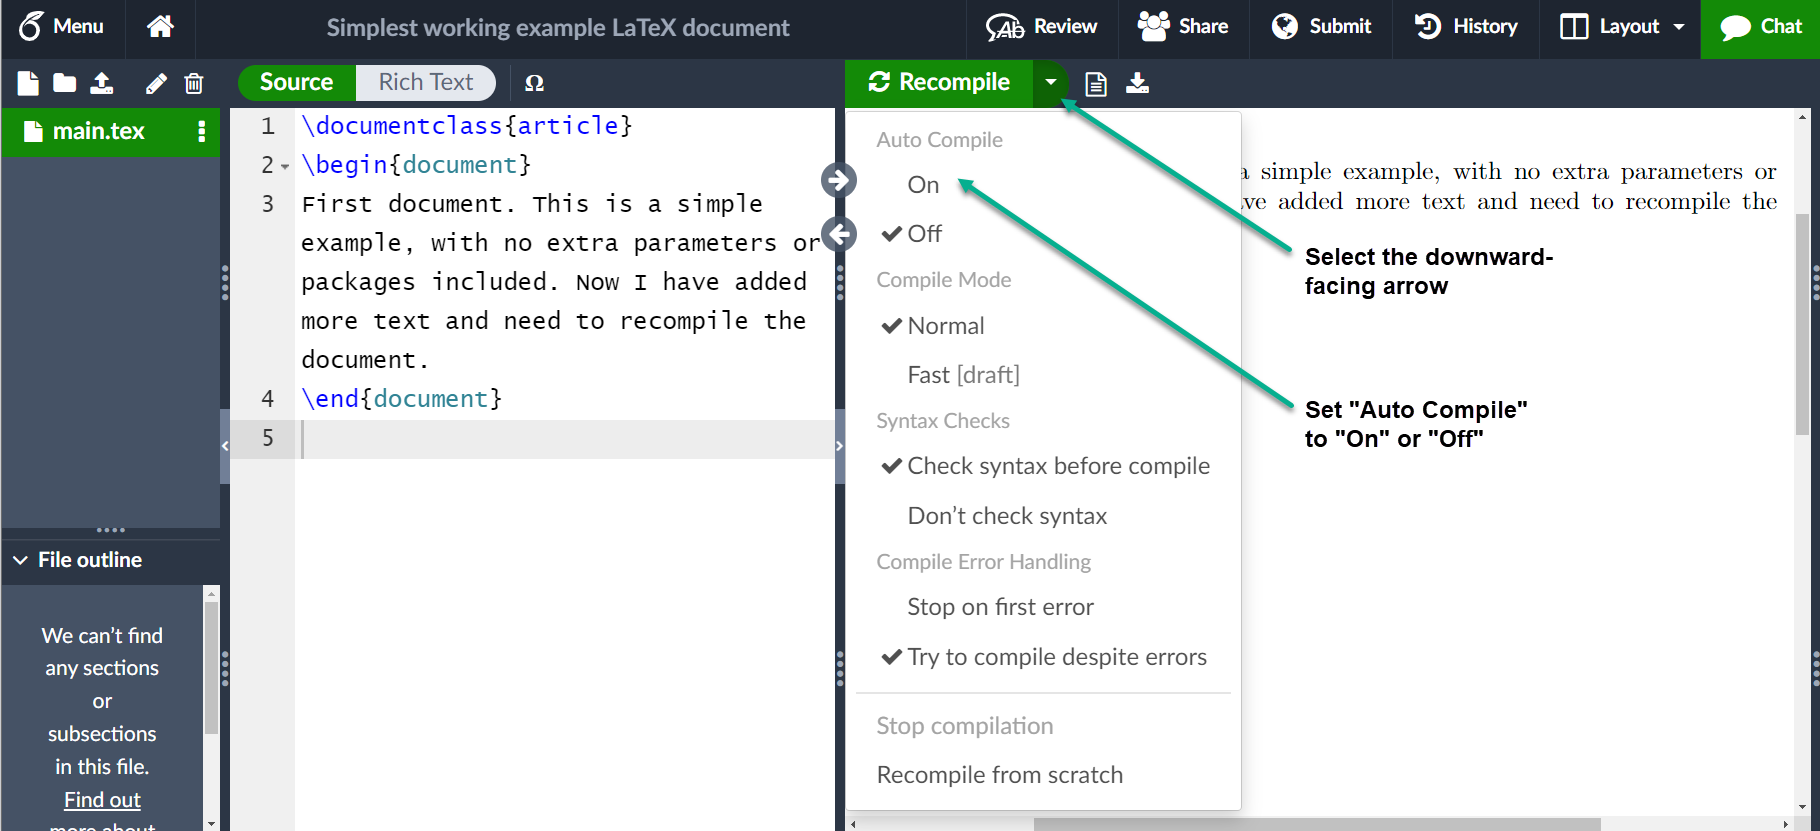
\includegraphics[width=\textwidth]{img3-1.png}

Having seen how to add content to our document, the next step is to give it a title. To do this, we must talk briefly about the \textbf{preamble}.